
\documentclass[sigplan,10pt,review]{acmart}

%% For double-blind review submission, w/ CCS and ACM Reference
%\documentclass[sigplan,10pt,review,anonymous]{acmart}\settopmatter{printfolios=true}
%% For single-blind review submission, w/o CCS and ACM Reference (max submission space)
%\documentclass[sigplan,10pt,review]{acmart}\settopmatter{printfolios=true,printccs=false,printacmref=false}
%% For single-blind review submission, w/ CCS and ACM Reference
%\documentclass[sigplan,10pt,review]{acmart}\settopmatter{printfolios=true}
%% For final camera-ready submission, w/ required CCS and ACM Reference
%\documentclass[sigplan,10pt]{acmart}\settopmatter{}

\settopmatter{printfolios=true,printccs=false,printacmref=false}

% TODO notes
%\usepackage[draft]{todonotes}
\usepackage{xcolor}
\newcommand\todo[1]{\textcolor{red}{\textbf{TODO:~}#1}}


%% Agda stuff
\usepackage[conor]{agda}
\newcommand{\AK}{\AgdaKeyword}
\newcommand{\AY}{\AgdaSymbol}
\newcommand{\AN}{\AgdaNumber}
\newcommand{\AS}{\AgdaSpace}
\newcommand{\AB}{\AgdaBound}
\newcommand{\AO}{\AgdaOperator}
\newcommand{\AI}{\AgdaInductiveConstructor}
\newcommand{\AC}{\AgdaCoinductiveConstructor}
\newcommand{\AD}{\AgdaDatatype}
\newcommand{\AF}{\AgdaFunction}
\newcommand{\AM}{\AgdaModule}
\newcommand{\AL}{\AgdaField}
\newcommand{\AR}{\AgdaArgument}
\newcommand{\AT}{\AgdaIndent}
\newcommand{\ARR}{\AgdaRecord}
\newcommand{\AP}{\AgdaPostulate}
\newcommand{\APT}{\AgdaPrimitiveType}


\newcommand{\nonterm}[1]{\hspace*{-0.1cm}\colorbox{orange!25}{#1}}
\newcommand{\hole}[1]{\colorbox{yellow!50}{\ensuremath{\bigbox_{#1}}}}
%% Conference information
%% Supplied to authors by publisher for camera-ready submission;
%% use defaults for review submission.
\acmConference[PL'17]{ACM SIGPLAN Conference on Programming Languages}{January 01--03, 2017}{New York, NY, USA}
\acmYear{2017}
\acmISBN{} % \acmISBN{978-x-xxxx-xxxx-x/YY/MM}
\acmDOI{} % \acmDOI{10.1145/nnnnnnn.nnnnnnn}
\startPage{1}

%% Copyright information
%% Supplied to authors (based on authors' rights management selection;
%% see authors.acm.org) by publisher for camera-ready submission;
%% use 'none' for review submission.
\setcopyright{none}
%\setcopyright{acmcopyright}
%\setcopyright{acmlicensed}
%\setcopyright{rightsretained}
%\copyrightyear{2017}           %% If different from \acmYear

%% Bibliography style
\bibliographystyle{ACM-Reference-Format}
%% Citation style
%\citestyle{acmauthoryear}  %% For author/year citations
%\citestyle{acmnumeric}     %% For numeric citations
%\setcitestyle{nosort}      %% With 'acmnumeric', to disable automatic
                            %% sorting of references within a single citation;
                            %% e.g., \cite{Smith99,Carpenter05,Baker12}
                            %% rendered as [14,5,2] rather than [2,5,14].
%\setcitesyle{nocompress}   %% With 'acmnumeric', to disable automatic
                            %% compression of sequential references within a
                            %% single citation;
                            %% e.g., \cite{Baker12,Baker14,Baker16}
                            %% rendered as [2,3,4] rather than [2-4].


%%%%%%%%%%%%%%%%%%%%%%%%%%%%%%%%%%%%%%%%%%%%%%%%%%%%%%%%%%%%%%%%%%%%%%
%% Note: Authors migrating a paper from traditional SIGPLAN
%% proceedings format to PACMPL format must update the
%% '\documentclass' and topmatter commands above; see
%% 'acmart-pacmpl-template.tex'.
%%%%%%%%%%%%%%%%%%%%%%%%%%%%%%%%%%%%%%%%%%%%%%%%%%%%%%%%%%%%%%%%%%%%%%
%% Some recommended packages.
\usepackage{booktabs}   %% For formal tables:
                        %% http://ctan.org/pkg/booktabs
\usepackage{subcaption} %% For complex figures with subfigures/subcaptions
                        %% http://ctan.org/pkg/subcaption
%% ODER: format ==         = "\mathrel{==}"
%% ODER: format /=         = "\neq "
%
%
\makeatletter
\@ifundefined{lhs2tex.lhs2tex.sty.read}%
  {\@namedef{lhs2tex.lhs2tex.sty.read}{}%
   \newcommand\SkipToFmtEnd{}%
   \newcommand\EndFmtInput{}%
   \long\def\SkipToFmtEnd#1\EndFmtInput{}%
  }\SkipToFmtEnd

\newcommand\ReadOnlyOnce[1]{\@ifundefined{#1}{\@namedef{#1}{}}\SkipToFmtEnd}
\usepackage{amstext}
\usepackage{amssymb}
\usepackage{stmaryrd}
\DeclareFontFamily{OT1}{cmtex}{}
\DeclareFontShape{OT1}{cmtex}{m}{n}
  {<5><6><7><8>cmtex8
   <9>cmtex9
   <10><10.95><12><14.4><17.28><20.74><24.88>cmtex10}{}
\DeclareFontShape{OT1}{cmtex}{m}{it}
  {<-> ssub * cmtt/m/it}{}
\newcommand{\texfamily}{\fontfamily{cmtex}\selectfont}
\DeclareFontShape{OT1}{cmtt}{bx}{n}
  {<5><6><7><8>cmtt8
   <9>cmbtt9
   <10><10.95><12><14.4><17.28><20.74><24.88>cmbtt10}{}
\DeclareFontShape{OT1}{cmtex}{bx}{n}
  {<-> ssub * cmtt/bx/n}{}
\newcommand{\tex}[1]{\text{\texfamily#1}}	% NEU

\newcommand{\Sp}{\hskip.33334em\relax}


\newcommand{\Conid}[1]{\mathit{#1}}
\newcommand{\Varid}[1]{\mathit{#1}}
\newcommand{\anonymous}{\kern0.06em \vbox{\hrule\@width.5em}}
\newcommand{\plus}{\mathbin{+\!\!\!+}}
\newcommand{\bind}{\mathbin{>\!\!\!>\mkern-6.7mu=}}
\newcommand{\rbind}{\mathbin{=\mkern-6.7mu<\!\!\!<}}% suggested by Neil Mitchell
\newcommand{\sequ}{\mathbin{>\!\!\!>}}
\renewcommand{\leq}{\leqslant}
\renewcommand{\geq}{\geqslant}
\usepackage{polytable}

%mathindent has to be defined
\@ifundefined{mathindent}%
  {\newdimen\mathindent\mathindent\leftmargini}%
  {}%

\def\resethooks{%
  \global\let\SaveRestoreHook\empty
  \global\let\ColumnHook\empty}
\newcommand*{\savecolumns}[1][default]%
  {\g@addto@macro\SaveRestoreHook{\savecolumns[#1]}}
\newcommand*{\restorecolumns}[1][default]%
  {\g@addto@macro\SaveRestoreHook{\restorecolumns[#1]}}
\newcommand*{\aligncolumn}[2]%
  {\g@addto@macro\ColumnHook{\column{#1}{#2}}}

\resethooks

\newcommand{\onelinecommentchars}{\quad-{}- }
\newcommand{\commentbeginchars}{\enskip\{-}
\newcommand{\commentendchars}{-\}\enskip}

\newcommand{\visiblecomments}{%
  \let\onelinecomment=\onelinecommentchars
  \let\commentbegin=\commentbeginchars
  \let\commentend=\commentendchars}

\newcommand{\invisiblecomments}{%
  \let\onelinecomment=\empty
  \let\commentbegin=\empty
  \let\commentend=\empty}

\visiblecomments

\newlength{\blanklineskip}
\setlength{\blanklineskip}{0.66084ex}

\newcommand{\hsindent}[1]{\quad}% default is fixed indentation
\let\hspre\empty
\let\hspost\empty
\newcommand{\NB}{\textbf{NB}}
\newcommand{\Todo}[1]{$\langle$\textbf{To do:}~#1$\rangle$}

\EndFmtInput
\makeatother
%
%
%
%
%
%
% This package provides two environments suitable to take the place
% of hscode, called "plainhscode" and "arrayhscode". 
%
% The plain environment surrounds each code block by vertical space,
% and it uses \abovedisplayskip and \belowdisplayskip to get spacing
% similar to formulas. Note that if these dimensions are changed,
% the spacing around displayed math formulas changes as well.
% All code is indented using \leftskip.
%
% Changed 19.08.2004 to reflect changes in colorcode. Should work with
% CodeGroup.sty.
%
\ReadOnlyOnce{polycode.fmt}%
\makeatletter

\newcommand{\hsnewpar}[1]%
  {{\parskip=0pt\parindent=0pt\par\vskip #1\noindent}}

% can be used, for instance, to redefine the code size, by setting the
% command to \small or something alike
\newcommand{\hscodestyle}{}

% The command \sethscode can be used to switch the code formatting
% behaviour by mapping the hscode environment in the subst directive
% to a new LaTeX environment.

\newcommand{\sethscode}[1]%
  {\expandafter\let\expandafter\hscode\csname #1\endcsname
   \expandafter\let\expandafter\endhscode\csname end#1\endcsname}

% "compatibility" mode restores the non-polycode.fmt layout.

\newenvironment{compathscode}%
  {\par\noindent
   \advance\leftskip\mathindent
   \hscodestyle
   \let\\=\@normalcr
   \let\hspre\(\let\hspost\)%
   \pboxed}%
  {\endpboxed\)%
   \par\noindent
   \ignorespacesafterend}

\newcommand{\compaths}{\sethscode{compathscode}}

% "plain" mode is the proposed default.
% It should now work with \centering.
% This required some changes. The old version
% is still available for reference as oldplainhscode.

\newenvironment{plainhscode}%
  {\hsnewpar\abovedisplayskip
   \advance\leftskip\mathindent
   \hscodestyle
   \let\hspre\(\let\hspost\)%
   \pboxed}%
  {\endpboxed%
   \hsnewpar\belowdisplayskip
   \ignorespacesafterend}

\newenvironment{oldplainhscode}%
  {\hsnewpar\abovedisplayskip
   \advance\leftskip\mathindent
   \hscodestyle
   \let\\=\@normalcr
   \(\pboxed}%
  {\endpboxed\)%
   \hsnewpar\belowdisplayskip
   \ignorespacesafterend}

% Here, we make plainhscode the default environment.

\newcommand{\plainhs}{\sethscode{plainhscode}}
\newcommand{\oldplainhs}{\sethscode{oldplainhscode}}
\plainhs

% The arrayhscode is like plain, but makes use of polytable's
% parray environment which disallows page breaks in code blocks.

\newenvironment{arrayhscode}%
  {\hsnewpar\abovedisplayskip
   \advance\leftskip\mathindent
   \hscodestyle
   \let\\=\@normalcr
   \(\parray}%
  {\endparray\)%
   \hsnewpar\belowdisplayskip
   \ignorespacesafterend}

\newcommand{\arrayhs}{\sethscode{arrayhscode}}

% The mathhscode environment also makes use of polytable's parray 
% environment. It is supposed to be used only inside math mode 
% (I used it to typeset the type rules in my thesis).

\newenvironment{mathhscode}%
  {\parray}{\endparray}

\newcommand{\mathhs}{\sethscode{mathhscode}}

% texths is similar to mathhs, but works in text mode.

\newenvironment{texthscode}%
  {\(\parray}{\endparray\)}

\newcommand{\texths}{\sethscode{texthscode}}

% The framed environment places code in a framed box.

\def\codeframewidth{\arrayrulewidth}
\RequirePackage{calc}

\newenvironment{framedhscode}%
  {\parskip=\abovedisplayskip\par\noindent
   \hscodestyle
   \arrayrulewidth=\codeframewidth
   \tabular{@{}|p{\linewidth-2\arraycolsep-2\arrayrulewidth-2pt}|@{}}%
   \hline\framedhslinecorrect\\{-1.5ex}%
   \let\endoflinesave=\\
   \let\\=\@normalcr
   \(\pboxed}%
  {\endpboxed\)%
   \framedhslinecorrect\endoflinesave{.5ex}\hline
   \endtabular
   \parskip=\belowdisplayskip\par\noindent
   \ignorespacesafterend}

\newcommand{\framedhslinecorrect}[2]%
  {#1[#2]}

\newcommand{\framedhs}{\sethscode{framedhscode}}

% The inlinehscode environment is an experimental environment
% that can be used to typeset displayed code inline.

\newenvironment{inlinehscode}%
  {\(\def\column##1##2{}%
   \let\>\undefined\let\<\undefined\let\\\undefined
   \newcommand\>[1][]{}\newcommand\<[1][]{}\newcommand\\[1][]{}%
   \def\fromto##1##2##3{##3}%
   \def\nextline{}}{\) }%

\newcommand{\inlinehs}{\sethscode{inlinehscode}}

% The joincode environment is a separate environment that
% can be used to surround and thereby connect multiple code
% blocks.

\newenvironment{joincode}%
  {\let\orighscode=\hscode
   \let\origendhscode=\endhscode
   \def\endhscode{\def\hscode{\endgroup\def\@currenvir{hscode}\\}\begingroup}
   %\let\SaveRestoreHook=\empty
   %\let\ColumnHook=\empty
   %\let\resethooks=\empty
   \orighscode\def\hscode{\endgroup\def\@currenvir{hscode}}}%
  {\origendhscode
   \global\let\hscode=\orighscode
   \global\let\endhscode=\origendhscode}%

\makeatother
\EndFmtInput
%

%% Agda keywords

%% Agda standard types

%% Constructors of the above types

%% Some standard functions
% format map    = "\AF{map}"       % Disabled

%% Non-colored stuff

%% Useful symbols


% fontsize of code snippets
\renewcommand\hscodestyle{%
   \setlength\leftskip{0.25cm}%
   \footnotesize
}

\begin{document}

\title{Verified and terminating dissections}

\author{Carlos Tom\'e Corti\~nas}
\affiliation{
  \department{Department of Information and Computing Sciences}  
  \institution{University of Utrecht}
  \country{The Netherlands}          
}
\email{first1.last1@inst1.edu}      

\author{Wouter Swierstra}
\affiliation{
  \department{Department of Information and Computing Sciences}
  \institution{University of Utrecht}
  \country{The Netherlands}
}
\email{w.s.swierstra@uu.nl}


\begin{abstract}
% The functional programming paradigm encourages a style of programming based on
%   the use of higher-order functions over inductively defined datatypes. A fold is
%   the prototypical example of such a function. However, its use for computation
%   comes at a price.  Folds for branching datatypes, such as binary trees, are by
%   definition not tail recursive functions.

%   McBride has proposed a method called
%   \emph{dissection}\cite{McBride:2008:CLM:1328438.1328474}, to
%   transform a fold into its tail-recursive counterpart. Nevertheless,
%   it is not clear why the resulting function terminates, nor it is
%   clear that the transformation preserves the fold's semantics. In
%   this paper we fill the gap by providing a fully machine checked
%   proof of the construction using the proof assistant Agda.
  \todo{Write abstract}
\end{abstract}


%% 2012 ACM Computing Classification System (CSS) concepts
%% Generate at 'http://dl.acm.org/ccs/ccs.cfm'.
\begin{CCSXML}
<ccs2012>
<concept>
<concept_id>10011007.10011006.10011008.10011009.10011012</concept_id>
<concept_desc>Software and its engineering~Functional languages</concept_desc>
<concept_significance>500</concept_significance>
</concept>
<concept>
<concept_id>10011007.10011006.10011008.10011024.10011028</concept_id>
<concept_desc>Software and its engineering~Data types and structures</concept_desc>
<concept_significance>300</concept_significance>
</concept>
<concept>
<concept_id>10011007.10011006.10011008.10011024.10011033</concept_id>
<concept_desc>Software and its engineering~Recursion</concept_desc>
<concept_significance>300</concept_significance>
</concept>
<concept>
<concept_id>10003752.10003753.10010622</concept_id>
<concept_desc>Theory of computation~Abstract machines</concept_desc>
<concept_significance>300</concept_significance>
</concept>
<concept>
<concept_id>10003752.10003790.10011740</concept_id>
<concept_desc>Theory of computation~Type theory</concept_desc>
<concept_significance>300</concept_significance>
</concept>
<concept>
<concept_id>10003752.10003790.10002990</concept_id>
<concept_desc>Theory of computation~Logic and verification</concept_desc>
<concept_significance>100</concept_significance>
</concept>
</ccs2012>
\end{CCSXML}

\ccsdesc[500]{Software and its engineering~Functional languages}
\ccsdesc[300]{Software and its engineering~Data types and structures}
\ccsdesc[300]{Software and its engineering~Recursion}
\ccsdesc[300]{Theory of computation~Abstract machines}
\ccsdesc[300]{Theory of computation~Type theory}
\ccsdesc[100]{Theory of computation~Logic and verification}

%% End of generated code


%% Keywords
%% comma separated list
\keywords{datatype generic programming, catamorphisms, dissection,
  dependent types, Agda, \todo{Keywords?}}


\maketitle



% Bound variables

\section{Introduction}

The type of binary trees is one of the most simple, yet widespread used,
datastructures in functional programming.  Beyond its elegance and simplicity,
in its definition lies an embarasing truth: a fold over a binary tree is not a
tail recursive function. In order to understand the problem, let us introduce
the type of binary trees.

\begin{hscode}\SaveRestoreHook
\column{B}{@{}>{\hspre}l<{\hspost}@{}}%
\column{3}{@{}>{\hspre}l<{\hspost}@{}}%
\column{5}{@{}>{\hspre}l<{\hspost}@{}}%
\column{10}{@{}>{\hspre}l<{\hspost}@{}}%
\column{13}{@{}>{\hspre}l<{\hspost}@{}}%
\column{19}{@{}>{\hspre}l<{\hspost}@{}}%
\column{E}{@{}>{\hspre}l<{\hspost}@{}}%
\>[3]{}\AK{data}\;\AD{Expr}\;\mathbin{:}\;\AP{Set}\;\AK{where}{}\<[E]%
\\
\>[3]{}\hsindent{2}{}\<[5]%
\>[5]{}\AI{Val}\;{}\<[10]%
\>[10]{}\mathbin{:}\;{}\<[13]%
\>[13]{}\AD{\ensuremath{\mathbb{N}}}\;{}\<[19]%
\>[19]{}\to \;\AD{Expr}{}\<[E]%
\\
\>[3]{}\hsindent{2}{}\<[5]%
\>[5]{}\AI{Add}\;{}\<[10]%
\>[10]{}\mathbin{:}\;{}\<[13]%
\>[13]{}\AD{Expr}\;{}\<[19]%
\>[19]{}\to \;\AD{Expr}\;\to \;\AD{Expr}{}\<[E]%
\ColumnHook
\end{hscode}\resethooks

We can write an evaluation function that maps binary trees to natural numbers if
we were to interpret the constructor \ensuremath{\AI{Add}} as addition.

\begin{hscode}\SaveRestoreHook
\column{B}{@{}>{\hspre}l<{\hspost}@{}}%
\column{3}{@{}>{\hspre}l<{\hspost}@{}}%
\column{21}{@{}>{\hspre}l<{\hspost}@{}}%
\column{E}{@{}>{\hspre}l<{\hspost}@{}}%
\>[3]{}\AF{eval}\;\mathbin{:}\;\AD{Expr}\;\to \;\AD{\ensuremath{\mathbb{N}}}{}\<[E]%
\\
\>[3]{}\AF{eval}\;(\AI{Val}\;\AB{n})\;{}\<[21]%
\>[21]{}\mathrel{=}\;\AB{n}{}\<[E]%
\\
\>[3]{}\AF{eval}\;(\AI{Add}\;\AB{\ensuremath{e_1}}\;\AB{\ensuremath{e_2}})\;{}\<[21]%
\>[21]{}\mathrel{=}\;\AF{eval}\;\AB{\ensuremath{e_1}}\;\AF{+}\;\AF{eval}\;\AB{\ensuremath{e_2}}{}\<[E]%
\ColumnHook
\end{hscode}\resethooks

The function \ensuremath{\AF{eval}} is compositional. The value of a node \ensuremath{\AI{Add}} is computed by
adding the values denoted by its subexpressions. And here lies the problem. The
operator \ensuremath{\AF{\_+\_}} needs both of its parameters to be evaluated before it can further
reduce. If the expression we want to compute over is very big this poses a
problem during runtime as the execution stack grows linearly with the size of
the input.

\todo[inline]{Maybe include something about Optimization through tco => get rid of
intermediate steps}

In order to solve the problem, we can make the execution stack explicit and
write a function that performs tail recursion over it. The idea is that we can
use a list to store both intemediate results and the subtress that still need to
be processed. We can define such a stack as follows:

\begin{hscode}\SaveRestoreHook
\column{B}{@{}>{\hspre}l<{\hspost}@{}}%
\column{3}{@{}>{\hspre}l<{\hspost}@{}}%
\column{5}{@{}>{\hspre}l<{\hspost}@{}}%
\column{12}{@{}>{\hspre}l<{\hspost}@{}}%
\column{20}{@{}>{\hspre}l<{\hspost}@{}}%
\column{E}{@{}>{\hspre}l<{\hspost}@{}}%
\>[3]{}\AK{data}\;\AD{Stack}\;\mathbin{:}\;\AP{Set}\;\AK{where}{}\<[E]%
\\
\>[3]{}\hsindent{2}{}\<[5]%
\>[5]{}\AI{Top}\;{}\<[12]%
\>[12]{}\mathbin{:}\;\AD{Stack}{}\<[E]%
\\
\>[3]{}\hsindent{2}{}\<[5]%
\>[5]{}\AI{Left}\;{}\<[12]%
\>[12]{}\mathbin{:}\;\AD{Expr}\;{}\<[20]%
\>[20]{}\to \;\AD{Stack}\;\to \;\AD{Stack}{}\<[E]%
\\
\>[3]{}\hsindent{2}{}\<[5]%
\>[5]{}\AI{Right}\;{}\<[12]%
\>[12]{}\mathbin{:}\;\AD{\ensuremath{\mathbb{N}}}\;{}\<[20]%
\>[20]{}\to \;\AD{Stack}\;\to \;\AD{Stack}{}\<[E]%
\ColumnHook
\end{hscode}\resethooks

Two mutually recursive functions that operate over the stack and tree are load
and unload. The former traverses a tree finding the leftmost leaf while the
latter dispathes over the stack by accumulating a partial result while looking
for the next subtree.

\begin{hscode}\SaveRestoreHook
\column{B}{@{}>{\hspre}l<{\hspost}@{}}%
\column{3}{@{}>{\hspre}l<{\hspost}@{}}%
\column{5}{@{}>{\hspre}l<{\hspost}@{}}%
\column{16}{@{}>{\hspre}l<{\hspost}@{}}%
\column{23}{@{}>{\hspre}l<{\hspost}@{}}%
\column{32}{@{}>{\hspre}l<{\hspost}@{}}%
\column{E}{@{}>{\hspre}l<{\hspost}@{}}%
\>[3]{}\AK{mutual}{}\<[E]%
\\
\>[3]{}\hsindent{2}{}\<[5]%
\>[5]{}\nonterm{\AF{load}}\;\mathbin{:}\;\AD{Expr}\;\to \;\AD{Stack}\;\to \;\AD{\ensuremath{\mathbb{N}}}{}\<[E]%
\\
\>[3]{}\hsindent{2}{}\<[5]%
\>[5]{}\AF{load}\;(\AI{Val}\;\AB{n})\;{}\<[23]%
\>[23]{}\AB{stk}\;\mathrel{=}\;\nonterm{\AF{unload}}\;\AB{n}\;\AB{stk}{}\<[E]%
\\
\>[3]{}\hsindent{2}{}\<[5]%
\>[5]{}\AF{load}\;(\AI{Add}\;\AB{\ensuremath{e_1}}\;\AB{\ensuremath{e_2}})\;{}\<[23]%
\>[23]{}\AB{stk}\;\mathrel{=}\;\nonterm{\AF{load}}\;\AB{\ensuremath{e_1}}\;(\AI{Left}\;\AB{\ensuremath{e_2}}\;\AB{stk}){}\<[E]%
\\[\blanklineskip]%
\>[3]{}\hsindent{2}{}\<[5]%
\>[5]{}\nonterm{\AF{unload}}\;\mathbin{:}\;\AD{\ensuremath{\mathbb{N}}}\;\to \;\AD{Stack}\;\to \;\AD{\ensuremath{\mathbb{N}}}{}\<[E]%
\\
\>[3]{}\hsindent{2}{}\<[5]%
\>[5]{}\AF{unload}\;\AB{v}\;{}\<[16]%
\>[16]{}\AI{Top}\;{}\<[32]%
\>[32]{}\mathrel{=}\;\AB{v}{}\<[E]%
\\
\>[3]{}\hsindent{2}{}\<[5]%
\>[5]{}\AF{unload}\;\AB{v}\;{}\<[16]%
\>[16]{}(\AI{Right}\;\AB{v'}\;\AB{stk})\;{}\<[32]%
\>[32]{}\mathrel{=}\;\nonterm{\AF{unload}}\;(\AB{v'}\;\AF{+}\;\AB{v})\;\AB{stk}{}\<[E]%
\\
\>[3]{}\hsindent{2}{}\<[5]%
\>[5]{}\AF{unload}\;\AB{v}\;{}\<[16]%
\>[16]{}(\AI{Left}\;\AB{r}\;\AB{stk})\;{}\<[32]%
\>[32]{}\mathrel{=}\;\nonterm{\AF{load}}\;\AB{r}\;(\AI{Right}\;\AB{v}\;\AB{stk}){}\<[E]%
\ColumnHook
\end{hscode}\resethooks

A tail recursive version of \ensuremath{\AF{eval}} can is defined by calling load with the empty
stack.

\begin{hscode}\SaveRestoreHook
\column{B}{@{}>{\hspre}l<{\hspost}@{}}%
\column{3}{@{}>{\hspre}l<{\hspost}@{}}%
\column{E}{@{}>{\hspre}l<{\hspost}@{}}%
\>[3]{}\AF{tail\text{-}rec\text{-}eval}\;\mathbin{:}\;\AD{Expr}\;\Varid{→}\;\AD{\ensuremath{\mathbb{N}}}{}\<[E]%
\\
\>[3]{}\AF{tail\text{-}rec\text{-}eval}\;\AB{e}\;\mathrel{=}\;\AF{load}\;\AB{e}\;\AI{Top}{}\<[E]%
\ColumnHook
\end{hscode}\resethooks

The reader might have noticed that the names of unload and load are higlighted
with \nonterm{orange}. This is because Agda's termination checker flags the pair of
functions as possibly non-terminating. Indeed, the recursive calls are not
always performed over syntactically smaller arguments. If we assumed that it
terminates we still do not know if it is correct in the sense that for every
input \ensuremath{\AF{tail\text{-}rec\text{-}eval}} and \ensuremath{\AF{eval}} agree on the output.

\begin{hscode}\SaveRestoreHook
\column{B}{@{}>{\hspre}l<{\hspost}@{}}%
\column{3}{@{}>{\hspre}l<{\hspost}@{}}%
\column{E}{@{}>{\hspre}l<{\hspost}@{}}%
\>[3]{}\AF{correct}\;\mathbin{:}\;\forall\;(\AB{e}\;\mathbin{:}\;\AD{Expr})\;\to \;\AF{eval}\;\AB{e}\;\AD{\ensuremath{\equiv}}\;\AF{tail\text{-}rec\text{-}eval}\;\AB{e}{}\<[E]%
\\
\>[3]{}\AF{correct}\;\mathrel{=}\;\hole{0}{}\<[E]%
\ColumnHook
\end{hscode}\resethooks

The main contribution of this paper is to show that we can both prove
termination and correctness of the construction in Agda. Specifically we show
how we can encode an ordering relation over stacks, show that the relation is
well founded and use it to define a tail recursive fold by structural recursion.
We discuss what are the main challenges that we have to overcome to convinde
Agda's termination checker that indeed something `goes smaller`. Moreover, our
approach allows us to get correctness almost for free.

McBride's insight is that we can calculate the type of stacks from the generic
description of a datatype by using Leibniz rules for derivatives. In later
sections of the paper, we discuss how to generalize our results to regular tree
datatypes and by doing so we show that McBride's intuition that the construction
is correct was true.

\section{Basic idea}

The functions \ensuremath{\AF{load}} and \ensuremath{\AF{unload}} are marked as non terminating because they are
not defined by structural recursion over their arguments. In particular, the
stack passed as an argument to the recursive call of \ensuremath{\AF{load}} in the definition of
\ensuremath{\AF{unload}} is structurally equal in size as the input stack.

Intuitively, \ensuremath{\AF{load}} and \ensuremath{\AF{unload}} fold the tree by traversing it from its
leftmost leaf to its rightmost using the stack to store both partial results and
the remaining subtrees to fold them as neccesary. The problem arises because the
stack is simply typed and any information about how the subtrees kept in the
stack relate to each other and to the original tree is lost once a subtree is
inserted onto the stack.

However, it is clear that virtually every node (either leaf or not) from the
original tree is visited at most twice during the computation. First when the
function \ensuremath{\AF{load}} decomposes it looking for its leftmost leaf and a second time
when \ensuremath{\AF{unload}} is accumulating over the stack searching for another subtree to
continue. This process is depicted in figure 1.

\begin{figure}[h]
  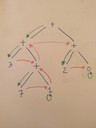
\includegraphics[scale=0.25]{figure1}
\end{figure}

We can argue that because there are finitely many nodes on a tree, \ensuremath{\AF{load}} and
\ensuremath{\AF{unload}} neccesarily terminate. The question is now, How can we encode this
information in such a way that Agda understand that the fold terminates?

The idea is that \ensuremath{\AF{load}} and \ensuremath{\AF{unload}} should not fold  the full input tree in one
go, but instead they will perform one step of the computation at a time.
Morover, by defining them by structural recursion over their arguments now they
are classified as terminating by the termination checker.

\begin{hscode}\SaveRestoreHook
\column{B}{@{}>{\hspre}l<{\hspost}@{}}%
\column{3}{@{}>{\hspre}l<{\hspost}@{}}%
\column{14}{@{}>{\hspre}l<{\hspost}@{}}%
\column{21}{@{}>{\hspre}l<{\hspost}@{}}%
\column{30}{@{}>{\hspre}l<{\hspost}@{}}%
\column{E}{@{}>{\hspre}l<{\hspost}@{}}%
\>[3]{}\AF{load}\;\mathbin{:}\;\AD{Expr}\;\to \;\AD{Stack}\;\to \;\AD{\ensuremath{\mathbb{N}}}\;\AF{\ensuremath{\times}}\;\AD{Stack}{}\<[E]%
\\
\>[3]{}\AF{load}\;(\AI{Val}\;\AB{n})\;{}\<[21]%
\>[21]{}\AB{stk}\;\mathrel{=}\;(\AB{n}\;\Varid{,}\;\AB{stk}){}\<[E]%
\\
\>[3]{}\AF{load}\;(\AI{Add}\;\AB{\ensuremath{e_1}}\;\AB{\ensuremath{e_2}})\;{}\<[21]%
\>[21]{}\AB{stk}\;\mathrel{=}\;\AF{load}\;\AB{\ensuremath{e_1}}\;(\AI{Left}\;\AB{\ensuremath{e_2}}\;\AB{stk}){}\<[E]%
\\[\blanklineskip]%
\>[3]{}\AF{unload}\;\mathbin{:}\;\AD{\ensuremath{\mathbb{N}}}\;\to \;\AD{Stack}\;\to \;(\AD{\ensuremath{\mathbb{N}}}\;\AF{\ensuremath{\times}}\;\AD{Stack})\;\AD{\ensuremath{\uplus}}\;\AD{\ensuremath{\mathbb{N}}}{}\<[E]%
\\
\>[3]{}\AF{unload}\;\AB{v}\;{}\<[14]%
\>[14]{}\AI{Top}\;{}\<[30]%
\>[30]{}\mathrel{=}\;\AI{inj\ensuremath{_2}}\;\AB{v}{}\<[E]%
\\
\>[3]{}\AF{unload}\;\AB{v}\;{}\<[14]%
\>[14]{}(\AI{Right}\;\AB{v'}\;\AB{stk})\;{}\<[30]%
\>[30]{}\mathrel{=}\;\AF{unload}\;(\AB{v'}\;\AF{+}\;\AB{v})\;\AB{stk}{}\<[E]%
\\
\>[3]{}\AF{unload}\;\AB{v}\;{}\<[14]%
\>[14]{}(\AI{Left}\;\AB{r}\;\AB{stk})\;{}\<[30]%
\>[30]{}\mathrel{=}\;\AI{inj\ensuremath{_1}}\;(\AF{load}\;\AB{r}\;(\AI{Right}\;\AB{v}\;\AB{stk})){}\<[E]%
\ColumnHook
\end{hscode}\resethooks

For example, if we take the same tree in figure 1, after \ensuremath{\AF{load}} finds the
initial leftmost leaf we can apply one step of the new \ensuremath{\AF{unload}} that will end up
in the next leaf to the right.


\begin{figure}[h]
  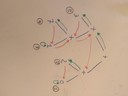
\includegraphics[scale=0.25]{figure2}
\end{figure}

A tail recursive fold corrensponds to repeatedly applying the function \ensuremath{\AF{unload}}
until we find a \ensuremath{\AI{inj\ensuremath{_2}}} whose value is the result of folding the tree.

\begin{hscode}\SaveRestoreHook
\column{B}{@{}>{\hspre}l<{\hspost}@{}}%
\column{3}{@{}>{\hspre}l<{\hspost}@{}}%
\column{5}{@{}>{\hspre}l<{\hspost}@{}}%
\column{7}{@{}>{\hspre}l<{\hspost}@{}}%
\column{E}{@{}>{\hspre}l<{\hspost}@{}}%
\>[3]{}\AF{tail\text{-}rec\text{-}eval}\;\mathbin{:}\;\AD{Expr}\;\to \;\AD{\ensuremath{\mathbb{N}}}{}\<[E]%
\\
\>[3]{}\AF{tail\text{-}rec\text{-}eval}\;\AB{e}\;\mathrel{=}\;\AF{rec}\;(\AF{load}\;\AB{e}\;\AI{Top}){}\<[E]%
\\
\>[3]{}\hsindent{2}{}\<[5]%
\>[5]{}\AK{where}{}\<[E]%
\\
\>[5]{}\hsindent{2}{}\<[7]%
\>[7]{}\nonterm{\AF{rec}}\;\mathbin{:}\;(\AD{\ensuremath{\mathbb{N}}}\;\AF{\ensuremath{\times}}\;\AD{Stack})\;\to \;\AD{\ensuremath{\mathbb{N}}}{}\<[E]%
\\
\>[5]{}\hsindent{2}{}\<[7]%
\>[7]{}\AF{rec}\;(\AB{n}\;\Varid{,}\;\AB{stk})\;\AK{with}\;\AF{unload}\;\AB{n}\;\AB{stk}{}\<[E]%
\\
\>[5]{}\hsindent{2}{}\<[7]%
\>[7]{}\Varid{...}\;\mid \;\AI{inj\ensuremath{_1}}\;\AB{z'}\;\mathrel{=}\;\nonterm{\AF{rec}}\;\AB{z'}{}\<[E]%
\\
\>[5]{}\hsindent{2}{}\<[7]%
\>[7]{}\Varid{...}\;\mid \;\AI{inj\ensuremath{_2}}\;\AB{r}\;\mathrel{=}\;\AB{r}{}\<[E]%
\ColumnHook
\end{hscode}\resethooks

The function \ensuremath{\AF{tail\text{-}rec\text{-}eval}} still does not pass the termination checker, The
variable \ensuremath{\AB{z'}} is not structurally smaller than \ensuremath{(\AB{n}\;\Varid{,}\;\AB{stk})}. However, now we can
refine it by using well founded recursion to make it structurally recursive by
performing the recursion over the accessibility predicate instead of the pair
\ensuremath{\AD{\ensuremath{\mathbb{N}}}\;\AF{\ensuremath{\times}}\;\AD{Stack}}.

\begin{hscode}\SaveRestoreHook
\column{B}{@{}>{\hspre}l<{\hspost}@{}}%
\column{3}{@{}>{\hspre}l<{\hspost}@{}}%
\column{5}{@{}>{\hspre}l<{\hspost}@{}}%
\column{7}{@{}>{\hspre}l<{\hspost}@{}}%
\column{E}{@{}>{\hspre}l<{\hspost}@{}}%
\>[3]{}\AF{tail\text{-}rec\text{-}eval}\;\mathbin{:}\;\AD{Expr}\;\to \;\AD{\ensuremath{\mathbb{N}}}{}\<[E]%
\\
\>[3]{}\AF{tail\text{-}rec\text{-}eval}\;\AB{e}\;\mathrel{=}\;\AF{rec}\;(\AF{load}\;\AB{e}\;\AI{Top})\;\hole{1}{}\<[E]%
\\
\>[3]{}\hsindent{2}{}\<[5]%
\>[5]{}\AK{where}{}\<[E]%
\\
\>[5]{}\hsindent{2}{}\<[7]%
\>[7]{}\AF{rec}\;\mathbin{:}\;(\AB{z}\;\mathbin{:}\;\AD{\ensuremath{\mathbb{N}}}\;\AF{\ensuremath{\times}}\;\AD{Stack})\;\to \;\AD{Acc}\;\AD{\_<\_}\;\AB{z}\;\to \;\AD{\ensuremath{\mathbb{N}}}{}\<[E]%
\\
\>[5]{}\hsindent{2}{}\<[7]%
\>[7]{}\AF{rec}\;(\AB{n}\;\Varid{,}\;\AB{stk})\;(\AI{acc}\;\Varid{rs})\;\AK{with}\;\AF{unload}\;\AB{n}\;\AB{stk}{}\<[E]%
\\
\>[5]{}\hsindent{2}{}\<[7]%
\>[7]{}\Varid{...}\;\mid \;\AI{inj\ensuremath{_1}}\;\AB{z'}\;\mathrel{=}\;\AF{rec}\;\AB{z'}\;(\Varid{rs}\;\hole{2}){}\<[E]%
\\
\>[5]{}\hsindent{2}{}\<[7]%
\>[7]{}\Varid{...}\;\mid \;\AI{inj\ensuremath{_2}}\;\AB{r}\;\mathrel{=}\;\AB{r}{}\<[E]%
\ColumnHook
\end{hscode}\resethooks

For the function above to work, we need to find a suitable definition for the
relation \ensuremath{\AD{\_<\_}} over pairs of \ensuremath{\AD{\ensuremath{\mathbb{N}}}\;\AF{\ensuremath{\times}}\;\AD{Stack}}, prove that applying \ensuremath{\AF{unload}}
results in an smaller element by the relation and finally show that the relation
is \ensuremath{\AF{Well\text{-}founded}}, so the call to \ensuremath{\AF{rec}} can be made in the first place. Before
any of that, we need to revisit Huet's notion of \emph{Zipper} and show how it
relates to what we are trying to achieve.

\subsection{Zippers up, Zippers down}

Huet introduced \emph{Zippers} to allow a tree datastructure to be efficiently
updated in a purely functional way. The idea is that any location on a tree,
either an internal node or a leaf, can be represented by a path to the root and
the subtree that hangs downwards.

The pair \ensuremath{\AD{\ensuremath{\mathbb{N}}}\;\AF{\ensuremath{\times}}\;\AD{Stack}} used to compute the tail recursive fold is nothing more
that a restricted version of the \emph{Zipper} where the locations can only be
leaves of the tree.

\begin{hscode}\SaveRestoreHook
\column{B}{@{}>{\hspre}l<{\hspost}@{}}%
\column{3}{@{}>{\hspre}l<{\hspost}@{}}%
\column{E}{@{}>{\hspre}l<{\hspost}@{}}%
\>[3]{}\AD{Zipper}\;\mathbin{:}\;\AP{Set}{}\<[E]%
\\
\>[3]{}\AD{Zipper}\;\mathrel{=}\;\AD{\ensuremath{\mathbb{N}}}\;\AF{\ensuremath{\times}}\;\AD{Stack}{}\<[E]%
\ColumnHook
\end{hscode}\resethooks

From a \ensuremath{\AD{Zipper}} we have to be able to reconstruct the original \ensuremath{\AD{Expr}} which
will be neccesary later on for the proof that the relation is well founded. For
this matter, we have to enhance the type of stacks to store not only the partial
results but also the expressions that where consumed in order to produce them.

\begin{hscode}\SaveRestoreHook
\column{B}{@{}>{\hspre}l<{\hspost}@{}}%
\column{3}{@{}>{\hspre}l<{\hspost}@{}}%
\column{25}{@{}>{\hspre}l<{\hspost}@{}}%
\column{26}{@{}>{\hspre}l<{\hspost}@{}}%
\column{27}{@{}>{\hspre}l<{\hspost}@{}}%
\column{E}{@{}>{\hspre}l<{\hspost}@{}}%
\>[3]{}\AD{Stack}\;\mathbin{:}\;\AP{Set}{}\<[E]%
\\
\>[3]{}\AD{Stack}\;\mathrel{=}\;\AD{List}\;(\AD{Expr}\;\AD{\ensuremath{\uplus}}\;{}\<[26]%
\>[26]{}(\AD{\ensuremath{\Sigma}}\;\AD{\ensuremath{\mathbb{N}}}\;\AK{\ensuremath{\lambda}}\;\AB{n}\;\to {}\<[E]%
\\
\>[26]{}\hsindent{1}{}\<[27]%
\>[27]{}\AD{\ensuremath{\Sigma}}\;\AD{Expr}\;\AK{\ensuremath{\lambda}}\;\AB{e}\;\to \;\AF{eval}\;\AB{e}\;\AD{\ensuremath{\equiv}}\;\AB{n})){}\<[E]%
\\
\>[3]{}\AK{pattern}\;\AI{Left}\;\AB{\ensuremath{t}}\;{}\<[25]%
\>[25]{}\mathrel{=}\;\AI{inj\ensuremath{_1}}\;\AB{\ensuremath{t}}{}\<[E]%
\\
\>[3]{}\AK{pattern}\;\AI{Right}\;\AB{n}\;\AB{\ensuremath{t}}\;\AB{\ensuremath{eq}}\;{}\<[25]%
\>[25]{}\mathrel{=}\;\AI{inj\ensuremath{_2}}\;(\AB{n}\;\Varid{,}\;\AB{\ensuremath{t}}\;\Varid{,}\;\AB{\ensuremath{eq}}){}\<[E]%
\ColumnHook
\end{hscode}\resethooks

The original expression for which a \ensuremath{\AD{\ensuremath{\mathbb{N}}}\;\AF{\ensuremath{\times}}\;\AD{Stack}} represents a position can be
reconstructed by forgeting that some part has already been evaluated.

\begin{hscode}\SaveRestoreHook
\column{B}{@{}>{\hspre}l<{\hspost}@{}}%
\column{3}{@{}>{\hspre}l<{\hspost}@{}}%
\column{27}{@{}>{\hspre}l<{\hspost}@{}}%
\column{36}{@{}>{\hspre}l<{\hspost}@{}}%
\column{E}{@{}>{\hspre}l<{\hspost}@{}}%
\>[3]{}\AF{plug\ensuremath{\Uparrow}}\;\mathbin{:}\;\AD{Expr}\;\to \;\AD{Stack}\;\to \;\AD{Expr}{}\<[E]%
\\
\>[3]{}\AF{plug\ensuremath{\Uparrow}}\;\AB{e}\;\AI{[]}\;{}\<[36]%
\>[36]{}\mathrel{=}\;\AB{e}{}\<[E]%
\\
\>[3]{}\AF{plug\ensuremath{\Uparrow}}\;\AB{e}\;(\AI{Left}\;\AB{\ensuremath{t}}\;{}\<[27]%
\>[27]{}\hspace{.4em}\AI{:\hspace{-.1em}:}\hspace{.4em}\;\AB{stk})\;{}\<[36]%
\>[36]{}\mathrel{=}\;\AF{plug\ensuremath{\Uparrow}}\;(\AI{Add}\;\AB{e}\;\AB{\ensuremath{t}})\;\AB{stk}{}\<[E]%
\\
\>[3]{}\AF{plug\ensuremath{\Uparrow}}\;\AB{e}\;(\AI{Right}\;\AB{n}\;\AB{\ensuremath{t}}\;\AB{\ensuremath{eq}}\;{}\<[27]%
\>[27]{}\hspace{.4em}\AI{:\hspace{-.1em}:}\hspace{.4em}\;\AB{stk})\;{}\<[36]%
\>[36]{}\mathrel{=}\;\AF{plug\ensuremath{\Uparrow}}\;(\AI{Add}\;\AB{\ensuremath{t}}\;\AB{e})\;\AB{stk}{}\<[E]%
\\[\blanklineskip]%
\>[3]{}\AF{plugZ\ensuremath{\Uparrow}}\;\mathbin{:}\;(\AD{\ensuremath{\mathbb{N}}}\;\AF{\ensuremath{\times}}\;\AD{Stack})\;\to \;\AD{Expr}{}\<[E]%
\\
\>[3]{}\AF{plugZ\ensuremath{\Uparrow}}\;(\AB{n}\;\Varid{,}\;\AB{stk})\;\mathrel{=}\;\AF{plug\ensuremath{\Uparrow}}\;(\AI{Val}\;\AB{n})\;\AB{stk}{}\<[E]%
\ColumnHook
\end{hscode}\resethooks

Our goal is to impose an ordering relation over elements of \ensuremath{\AD{Zipper}} such that
for any input the \ensuremath{\AF{unload}} function delivers a \ensuremath{\AD{Zipper}} that is smaller by the
relation when it does not terminate with a value. Because the folding happens
from left to right, we want the relation to order the leaves of the tree
accordingly, so the leftmost leaf is the greatest element and the rightmost the
smallest. Using the example from before, we number the leaves as follows:

\begin{figure}[h]
  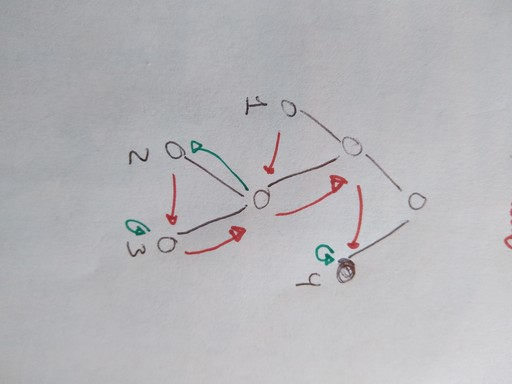
\includegraphics[scale=0.25, angle=90]{figure3}
\end{figure}

Using the \ensuremath{\AD{Stack}} as a path from the leaf to the root of the tree is difficult
if not impossible to encode a smaller than relation that does not relate any two
elements. Such relation has to be defined by induction on the \ensuremath{\AD{Stack}} part of the
\ensuremath{\AD{Zipper}}. But for any two given stacks a priori we cannot know how many layers
we have to peel in order to reach a case where one of them is obviously smaller
that the other.

We can approach the problem by understanding the \ensuremath{\AD{Stack}} not as a path from the
leaf up to the root but from the root down to the leaf. This change of
perspective is realised with a new plug function that does the opposite of
\ensuremath{\AF{plug\ensuremath{\Uparrow}}}.

\begin{hscode}\SaveRestoreHook
\column{B}{@{}>{\hspre}l<{\hspost}@{}}%
\column{3}{@{}>{\hspre}l<{\hspost}@{}}%
\column{28}{@{}>{\hspre}l<{\hspost}@{}}%
\column{37}{@{}>{\hspre}l<{\hspost}@{}}%
\column{E}{@{}>{\hspre}l<{\hspost}@{}}%
\>[3]{}\AF{plug\ensuremath{\Downarrow}}\;\mathbin{:}\;\AD{Expr}\;\to \;\AD{Stack}\;\to \;\AD{Expr}{}\<[E]%
\\
\>[3]{}\AF{plug\ensuremath{\Downarrow}}\;\AB{e}\;\AI{[]}\;{}\<[37]%
\>[37]{}\mathrel{=}\;\AB{e}{}\<[E]%
\\
\>[3]{}\AF{plug\ensuremath{\Downarrow}}\;\AB{e}\;(\AI{Left}\;\AB{\ensuremath{t}}\;{}\<[28]%
\>[28]{}\hspace{.4em}\AI{:\hspace{-.1em}:}\hspace{.4em}\;\AB{stk})\;{}\<[37]%
\>[37]{}\mathrel{=}\;\AI{Add}\;(\AF{plug\ensuremath{\Downarrow}}\;\AB{e}\;\AB{stk})\;\AB{\ensuremath{t}}{}\<[E]%
\\
\>[3]{}\AF{plug\ensuremath{\Downarrow}}\;\AB{e}\;(\AI{Right}\;\AB{n}\;\anonymous \;\anonymous \;{}\<[28]%
\>[28]{}\hspace{.4em}\AI{:\hspace{-.1em}:}\hspace{.4em}\;\AB{stk})\;{}\<[37]%
\>[37]{}\mathrel{=}\;\AI{Add}\;\AB{\ensuremath{t}}\;(\AF{plug\ensuremath{\Downarrow}}\;\AB{e}\;\AB{stk}){}\<[E]%
\\[\blanklineskip]%
\>[3]{}\AF{plugZ\ensuremath{\Downarrow}}\;\mathbin{:}\;(\AD{\ensuremath{\mathbb{N}}}\;\AF{\ensuremath{\times}}\;\AD{Stack})\;\to \;\AD{Expr}{}\<[E]%
\\
\>[3]{}\AF{plugZ\ensuremath{\Downarrow}}\;(\AB{n}\;\Varid{,}\;\AB{stk})\;\mathrel{=}\;\AF{plug\ensuremath{\Downarrow}}\;(\AI{Val}\;\AB{n})\;\AB{stk}{}\<[E]%
\ColumnHook
\end{hscode}\resethooks

It is clear that both views of the \ensuremath{\AD{Zipper}} are related. Indeed, to transport
from one to the other we only have to reverse the stack. We show the equvalence
with the following lemma\footnote{The other way around only requires to use
BLABLA of \ensuremath{\AF{reverse}}}:

\begin{hscode}\SaveRestoreHook
\column{B}{@{}>{\hspre}l<{\hspost}@{}}%
\column{3}{@{}>{\hspre}l<{\hspost}@{}}%
\column{23}{@{}>{\hspre}l<{\hspost}@{}}%
\column{44}{@{}>{\hspre}l<{\hspost}@{}}%
\column{E}{@{}>{\hspre}l<{\hspost}@{}}%
\>[3]{}\AF{plug\ensuremath{\Downarrow}}\AF{\text{-}to\text{-}}\AF{plug\ensuremath{\Uparrow}}\;{}\<[23]%
\>[23]{}\mathbin{:}\;\forall\;(\AB{e}\;\mathbin{:}\;\AD{Expr})\;(\AB{stk}\;\mathbin{:}\;\AD{Stack}){}\<[E]%
\\
\>[23]{}\Varid{→}\;\AF{plug\ensuremath{\Downarrow}}\;\AB{e}\;\AB{stk}\;\AD{\ensuremath{\equiv}}\;{}\<[44]%
\>[44]{}\AF{plug\ensuremath{\Uparrow}}\;\AB{e}\;(\AF{reverse}\;\AB{stk}){}\<[E]%
\ColumnHook
\end{hscode}\resethooks


Why do we need this equivalence? The bottom up view of a \ensuremath{\AD{Zipper}} is suitable
for defining the tail recursive fold, alas to prove termination we have to use
use the top down view to describe the relation we need.

\subsection{A relation on Zipper}

The relation over elements of \ensuremath{\AD{Zipper}} is defined by induction on the \ensuremath{\AD{Stack}}.
If we start in the root of the tree, we can navigate downwards both stacks in
parallel removing their common prefix. Once we find an \ensuremath{\AI{Add}} where they
disagree then whether the first \ensuremath{\AD{Zipper}} is located in the left or right
subtree fully determines if its bigger or smaller than the other \ensuremath{\AD{Zipper}}.
The following type accounts for this explanation:

\begin{hscode}\SaveRestoreHook
\column{B}{@{}>{\hspre}l<{\hspost}@{}}%
\column{3}{@{}>{\hspre}l<{\hspost}@{}}%
\column{5}{@{}>{\hspre}l<{\hspost}@{}}%
\column{14}{@{}>{\hspre}l<{\hspost}@{}}%
\column{18}{@{}>{\hspre}l<{\hspost}@{}}%
\column{19}{@{}>{\hspre}l<{\hspost}@{}}%
\column{23}{@{}>{\hspre}l<{\hspost}@{}}%
\column{44}{@{}>{\hspre}l<{\hspost}@{}}%
\column{E}{@{}>{\hspre}l<{\hspost}@{}}%
\>[3]{}\AK{data}\;\AD{\_<\_}\;\mathbin{:}\;\AD{Zipper}\;\to \;\AD{Zipper}\;\to \;\AP{Set}\;\AK{where}{}\<[E]%
\\
\>[3]{}\hsindent{2}{}\<[5]%
\>[5]{}\AI{<\text{-}Right}\;{}\<[14]%
\>[14]{}\mathbin{:}\;(\AB{\ensuremath{t_1}}\;\Varid{,}\;\AB{\ensuremath{s_1}})\;\AD{<}\;(\AB{\ensuremath{t_2}}\;\Varid{,}\;\AB{\ensuremath{s_2}})\;{}\<[E]%
\\
\>[14]{}\to \;{}\<[18]%
\>[18]{}(\AB{\ensuremath{t_1}}\;\Varid{,}\;\AI{Right}\;\Varid{l}\;\AB{n}\;\AB{\ensuremath{eq}}\;\hspace{.4em}\AI{:\hspace{-.1em}:}\hspace{.4em}\;\AB{\ensuremath{s_1}})\;\AD{<}\;(\AB{\ensuremath{t_2}}\;\Varid{,}\;\AI{Right}\;\Varid{l}\;\AB{n}\;\AB{\ensuremath{eq}}\;\hspace{.4em}\AI{:\hspace{-.1em}:}\hspace{.4em}\;\AB{\ensuremath{s_2}}){}\<[E]%
\\
\>[3]{}\hsindent{2}{}\<[5]%
\>[5]{}\AI{<\text{-}Left}\;{}\<[14]%
\>[14]{}\mathbin{:}\;(\AB{\ensuremath{t_1}}\;\Varid{,}\;\AB{\ensuremath{s_1}})\;\AD{<}\;(\AB{\ensuremath{t_2}}\;\Varid{,}\;\AB{\ensuremath{s_2}})\;{}\<[E]%
\\
\>[14]{}\to \;{}\<[18]%
\>[18]{}(\AB{\ensuremath{t_1}}\;\Varid{,}\;\AI{Left}\;\AB{r}\;\hspace{.4em}\AI{:\hspace{-.1em}:}\hspace{.4em}\;\AB{\ensuremath{s_1}})\;{}\<[44]%
\>[44]{}\AD{<}\;(\AB{\ensuremath{t_2}}\;\Varid{,}\;\AI{Left}\;\AB{r}\;\hspace{.4em}\AI{:\hspace{-.1em}:}\hspace{.4em}\;\AB{\ensuremath{s_2}}){}\<[E]%
\\
\>[3]{}\hsindent{2}{}\<[5]%
\>[5]{}\AI{<\text{-}Right\text{-}Left}\;{}\<[19]%
\>[19]{}\mathbin{:}\;{}\<[23]%
\>[23]{}(\AB{\ensuremath{t_1}'}\;\AD{\ensuremath{\equiv}}\;\AF{plug\ensuremath{\Downarrow}}\;(\Conid{Tip}\;\AB{\ensuremath{t_2}})\;\AB{\ensuremath{s_2}})\;{}\<[E]%
\\
\>[19]{}\to \;{}\<[23]%
\>[23]{}(\AB{\ensuremath{t_2}'}\;\AD{\ensuremath{\equiv}}\;\AF{plug\ensuremath{\Downarrow}}\;(\Conid{Tip}\;\AB{\ensuremath{t_1}})\;\AB{\ensuremath{s_1}})\;{}\<[E]%
\\
\>[19]{}\to \;{}\<[23]%
\>[23]{}(\AB{\ensuremath{t_1}}\;\Varid{,}\;\AI{Right}\;\AB{n}\;\AB{\ensuremath{t_1}'}\;\AB{\ensuremath{eq}}\;\hspace{.4em}\AI{:\hspace{-.1em}:}\hspace{.4em}\;\AB{\ensuremath{s_1}})\;\AD{<}\;(\AB{\ensuremath{t_2}}\;\Varid{,}\;\AI{Left}\;\AB{\ensuremath{t_2}'}\;\hspace{.4em}\AI{:\hspace{-.1em}:}\hspace{.4em}\;\AB{\ensuremath{s_2}}){}\<[E]%
\ColumnHook
\end{hscode}\resethooks

Having the relation defined, we turn our focus to prove that it is well founded.
This is an important step towards filling the holes that were left open in the
function \ensuremath{\AF{tail\text{-}rec\text{-}eval}}.

A relation is well founded iff all the descending chains starting from an
arbitrary element are finite. In a theorem prover such as Agda, an alternative
definition of well foundedness is used which is based on an accesibility
predicate.

We can try to prove that the relation is well founded by using an auxiliary
function that allows us to pattern match on the smaller than proof. When doing
so, the inputs are refined to concrete constructors. Normally the proof either
makes use of recursion over the proof or over the input, but in the case of the
\ensuremath{\AI{<\text{-}Right\text{-}Left}} constructor we do not have either option, because the smaller
element is not structurally related to the bigger and the proof does not have
any recursive structure to use.

\begin{hscode}\SaveRestoreHook
\column{B}{@{}>{\hspre}l<{\hspost}@{}}%
\column{5}{@{}>{\hspre}l<{\hspost}@{}}%
\column{7}{@{}>{\hspre}l<{\hspost}@{}}%
\column{11}{@{}>{\hspre}l<{\hspost}@{}}%
\column{E}{@{}>{\hspre}l<{\hspost}@{}}%
\>[B]{}\Varid{<-WF}\;\mathbin{:}\;\AF{Well\text{-}founded}\;\AD{\_<\_}{}\<[E]%
\\
\>[B]{}\Varid{<-WF}\;\Varid{x}\;\mathrel{=}\;\AI{acc}\;(\Varid{aux}\;\Varid{x}){}\<[E]%
\\
\>[B]{}\hsindent{5}{}\<[5]%
\>[5]{}\AK{where}{}\<[E]%
\\
\>[5]{}\hsindent{2}{}\<[7]%
\>[7]{}\Varid{aux}\;\mathbin{:}\;\Varid{∀}\;(\Varid{x}\;\mathbin{:}\;\AD{Zipper})\;{}\<[E]%
\\
\>[7]{}\hsindent{4}{}\<[11]%
\>[11]{}\to \;\Varid{∀}\;(\Varid{y}\;\mathbin{:}\;\AD{Zipper})\;\to \;\Varid{y}\;\AD{<}\;\Varid{x}\;\to \;\AD{Acc}\;\AD{\_<\_}\;\Varid{y}{}\<[E]%
\\
\>[5]{}\hsindent{2}{}\<[7]%
\>[7]{}\Varid{aux}\;\AS{.}\hspace*{-0.1cm}\;(\AB{\ensuremath{t_2}}\;\Varid{,}\;\AI{Left}\;\AB{\ensuremath{t_1}'}\;\hspace{.4em}\AI{:\hspace{-.1em}:}\hspace{.4em}\;\AB{\ensuremath{s_2}})\;\AS{.}\hspace*{-0.1cm}\;(\AB{\ensuremath{t_1}}\;\Varid{,}\;\AI{Right}\;\AB{n}\;\AB{\ensuremath{t_2}'}\;\AB{\ensuremath{eq}}\;\hspace{.4em}\AI{:\hspace{-.1em}:}\hspace{.4em}\;\AB{\ensuremath{s_1}})\;(\AI{<\text{-}Right\text{-}Left}\;\Varid{eq1}\;\Varid{eq2})\;\mathrel{=}\;\{\mskip1.5mu \mathbin{!!}\mskip1.5mu\}{}\<[E]%
\\
\>[5]{}\hsindent{2}{}\<[7]%
\>[7]{}\Varid{aux}\;\Varid{...}{}\<[E]%
\ColumnHook
\end{hscode}\resethooks

The proof fails because in \ensuremath{\Varid{aux}} both Zippers \ensuremath{\Varid{x}} and \ensuremath{\Varid{y}} might very well be
locations of leaves belonging to different trees as far we know. Thanks to the
use of dependent types, the property that a Zipper represents a position inside a
concrete tree can be made explicit at the type level.

\begin{hscode}\SaveRestoreHook
\column{B}{@{}>{\hspre}l<{\hspost}@{}}%
\column{3}{@{}>{\hspre}l<{\hspost}@{}}%
\column{5}{@{}>{\hspre}l<{\hspost}@{}}%
\column{E}{@{}>{\hspre}l<{\hspost}@{}}%
\>[3]{}\AK{data}\;\AD{Zipper\ensuremath{\Downarrow}}\;(\AB{e}\;\mathbin{:}\;\AD{Expr})\;\mathbin{:}\;\AP{Set}\;\AK{where}{}\<[E]%
\\
\>[3]{}\hsindent{2}{}\<[5]%
\>[5]{}\Varid{\char92 \char95 ,\char92 \char95 }\;\mathbin{:}\;(\AB{z}\;\mathbin{:}\;\AD{Zipper})\;\to \;\AF{plugZ\ensuremath{\Downarrow}}\;\AB{z}\;\AD{\ensuremath{\equiv}}\;\AB{e}\;\to \;\AD{Zipper\ensuremath{\Downarrow}}\;\AB{e}{}\<[E]%
\ColumnHook
\end{hscode}\resethooks

We write a relation that is enforced to only relate Zippers beloging to the same
\ensuremath{\AD{Expr}} by using a common value of that type as an of \ensuremath{\AD{Zipper\ensuremath{\Downarrow}}}

\begin{hscode}\SaveRestoreHook
\column{B}{@{}>{\hspre}l<{\hspost}@{}}%
\column{3}{@{}>{\hspre}l<{\hspost}@{}}%
\column{5}{@{}>{\hspre}l<{\hspost}@{}}%
\column{E}{@{}>{\hspre}l<{\hspost}@{}}%
\>[3]{}\AK{data}\;\Conid{IxltOp}\;\mathbin{:}\;(\AB{e}\;\mathbin{:}\;\AD{Expr})\;\to \;\AD{Zipper\ensuremath{\Downarrow}}\;\AB{e}\;\to \;\AD{Zipper\ensuremath{\Downarrow}}\;\AB{e}\;\to \;\AP{Set}\;\AK{where}{}\<[E]%
\\
\>[3]{}\hsindent{2}{}\<[5]%
\>[5]{}\Varid{...}{}\<[E]%
\ColumnHook
\end{hscode}\resethooks

The concrete details of the relation follow very much the one we gave before,
with the exception that every case has attached a new piece of information
specifying the concrete \ensuremath{\AD{Expr}} obtained by plugging both Zippers.

The new version of the relation is suitable for proving well foundedness because
we can pattern match on the equality included in the \ensuremath{\AD{Zipper\ensuremath{\Downarrow}}} type to show how 
the overall structure decreases. This allows us to use the recursion we need to
complete the proof.
In particular, the case we were not able to prove before, now can be proven by learning that
\ensuremath{(\AB{\ensuremath{t_2}}\;\Varid{,}\;\AB{\ensuremath{s_2}})} is a position on the left subtree while \ensuremath{(\AB{\ensuremath{t_1}}\;\Varid{,}\;\AB{\ensuremath{s_1}})} is on the
right subtree of a common \ensuremath{\AI{Add}} node.

\begin{hscode}\SaveRestoreHook
\column{B}{@{}>{\hspre}l<{\hspost}@{}}%
\column{3}{@{}>{\hspre}l<{\hspost}@{}}%
\column{5}{@{}>{\hspre}l<{\hspost}@{}}%
\column{7}{@{}>{\hspre}l<{\hspost}@{}}%
\column{11}{@{}>{\hspre}l<{\hspost}@{}}%
\column{E}{@{}>{\hspre}l<{\hspost}@{}}%
\>[3]{}\Varid{<-WF}\;\mathbin{:}\;\forall\;\AB{e}\;\to \;\AF{Well\text{-}founded}\;(\Conid{IxltOp}\;\AB{e}){}\<[E]%
\\
\>[3]{}\Varid{<-WF}\;\Varid{x}\;\mathrel{=}\;\AI{acc}\;(\Varid{aux}\;\AB{e}\;\Varid{x}){}\<[E]%
\\
\>[3]{}\hsindent{2}{}\<[5]%
\>[5]{}\AK{where}{}\<[E]%
\\
\>[5]{}\hsindent{2}{}\<[7]%
\>[7]{}\Varid{aux}\;\mathbin{:}\;\forall\;(\AB{e}\;\mathbin{:}\;\AD{Expr})\;\to \;\forall\;(\Varid{x}\;\mathbin{:}\;\AD{Zipper\ensuremath{\Downarrow}}\;\AB{e}){}\<[E]%
\\
\>[7]{}\hsindent{4}{}\<[11]%
\>[11]{}\to \;\forall\;(\Varid{y}\;\mathbin{:}\;\AD{Zipper\ensuremath{\Downarrow}}\;\AB{e})\;\to \;\Varid{y}\;\AD{<}\;\Varid{x}\;\to \;\AD{Acc}\;(\Conid{IxltOp}\;\AB{e})\;\Varid{y}{}\<[E]%
\\
\>[5]{}\hsindent{2}{}\<[7]%
\>[7]{}\Varid{aux}\;\AS{.}\hspace*{-0.1cm}\;(\AI{Add}\;(\Varid{plug}))\;\AS{.}\hspace*{-0.1cm}\;((\AB{\ensuremath{t_2}}\;\Varid{,}\;\AI{Left}\;\AB{\ensuremath{t_1}'}\;\hspace{.4em}\AI{:\hspace{-.1em}:}\hspace{.4em}\;\AB{\ensuremath{s_2}}))\;\Varid{,}\;\AI{refl})\;\AS{.}\hspace*{-0.1cm}\;((\AB{\ensuremath{t_1}}\;\Varid{,}\;\AI{Right}\;\AB{n}\;\AB{\ensuremath{t_2}'}\;\AB{\ensuremath{eq}}\;\hspace{.4em}\AI{:\hspace{-.1em}:}\hspace{.4em}\;\AB{\ensuremath{s_1}})\;\Varid{,}\;\Varid{eq2})\;{}\<[E]%
\\
\>[7]{}\hsindent{4}{}\<[11]%
\>[11]{}(\AI{<\text{-}Right\text{-}Left}\;\Varid{eq1}\;\Varid{eq2})\;\mathrel{=}\;\{\mskip1.5mu \mathbin{!!}\mskip1.5mu\}\;{}\<[E]%
\\
\>[5]{}\hsindent{2}{}\<[7]%
\>[7]{}\Varid{aux}\;\Varid{...}{}\<[E]%
\ColumnHook
\end{hscode}\resethooks

We have now the proof of well foundedness for the relation defined over top-down Zippers. We also have proven that
there is an equivalence between top-down and bottom-up Zippers. We exploit it by using the top-down encoding for
the termination proof while we use the bottom-up to actually compute in a tail recursive manner.

Thus we prove a lemma stating that if we apply unload to a bottom-up Zipper and this results in another
Zipper, then the result is smaller by the relation than the input. However, to show it we have to 
convert them to the top down representation. In overall, what we have is the following lemma:

\begin{hscode}\SaveRestoreHook
\column{B}{@{}>{\hspre}l<{\hspost}@{}}%
\column{13}{@{}>{\hspre}l<{\hspost}@{}}%
\column{E}{@{}>{\hspre}l<{\hspost}@{}}%
\>[B]{}\Varid{unload-ltop}\;\mathbin{:}\;\forall\;\AB{n}\;\AB{\ensuremath{eq}}\;\Varid{s}\;\Varid{t'}\;\Varid{s'}\;\to \;\AF{unload}\;(\Conid{Tip}\;\AB{n})\;(\Conid{TipA}\;\AB{n})\;\AB{\ensuremath{eq}}\;\Varid{s}\;\AD{\ensuremath{\equiv}}\;\Varid{inj₁}\;(\Varid{t'}\;\Varid{,}\;\Varid{s'}){}\<[E]%
\\
\>[B]{}\hsindent{13}{}\<[13]%
\>[13]{}\to \;(\Varid{t'}\;\Varid{,}\;\AF{reverse}\;\Varid{s'})\;\AD{\_<\_}\;(\AB{n}\;\Varid{,}\;\AF{reverse}\;\Varid{s}){}\<[E]%
\ColumnHook
\end{hscode}\resethooks

\subsection{Correctness}

Indexing the \emph{Zipper} with an expression allow us to prove correcness of
the transformation easily. The expression during the fold does not change, thus
in every step of the computation the result of its evaluation remains constant.

By using induction over the definition of unload, we can prove that when \ensuremath{\AF{unload}} 
delivers a value, it corresponds to the result of evaluating of the input expression.
In order to do so, we enrich the type of \ensuremath{\AF{unload}} to include the expression that has already
been folded and we have its result. 

\begin{hscode}\SaveRestoreHook
\column{B}{@{}>{\hspre}l<{\hspost}@{}}%
\column{3}{@{}>{\hspre}l<{\hspost}@{}}%
\column{19}{@{}>{\hspre}l<{\hspost}@{}}%
\column{E}{@{}>{\hspre}l<{\hspost}@{}}%
\>[3]{}\AF{unload}\;\mathbin{:}\;(\AB{e}\;\mathbin{:}\;\AD{Expr})\;\to \;(\AB{n}\;\mathbin{:}\;\AD{\ensuremath{\mathbb{N}}})\;\to \;\AF{eval}\;\AB{e}\;\AD{\ensuremath{\equiv}}\;\AB{n}\;\to \;\AD{Stack}\;\to \;(\AD{\ensuremath{\mathbb{N}}}\;\AF{\ensuremath{\times}}\;\AD{Stack})\;\AD{\ensuremath{\uplus}}\;\AD{\ensuremath{\mathbb{N}}}{}\<[E]%
\\[\blanklineskip]%
\>[3]{}\Varid{unload-correct}\;{}\<[19]%
\>[19]{}\mathbin{:}\;\forall\;(\AB{e}\;\mathbin{:}\;\AD{Expr})\;(\AB{n}\;\mathbin{:}\;\AD{\ensuremath{\mathbb{N}}})\;(\AB{\ensuremath{eq}}\;\mathbin{:}\;\AF{eval}\;\AB{e}\;\AD{\ensuremath{\equiv}}\;\AB{n})\;(\Varid{s}\;\mathbin{:}\;\AD{Stack})\;(\Varid{x}\;\mathbin{:}\;\AD{\ensuremath{\mathbb{N}}}){}\<[E]%
\\
\>[19]{}\to \;\AF{unload}\;\AB{e}\;\AB{n}\;\AB{\ensuremath{eq}}\;\Varid{s}\;\Varid{≡}\;\AI{inj\ensuremath{_2}}\;\Varid{x}\;\to \;\AF{eval}\;\AB{e}\;\AD{\ensuremath{\equiv}}\;\Varid{x}{}\<[E]%
\ColumnHook
\end{hscode}\resethooks

Proving correctness of the whole transformation amounts to show that it holds for the
auxiliary recursor that we use to write the function \ensuremath{\AF{tail\text{-}rec\text{-}eval}}. We use well founded 
recursion to do structural recursion over the accesibility predicate and use the lemma 
\ensuremath{\Varid{unload-correct}} in the base case.

\todo[inline]{STOP HERE}

\section{Regular universe}
  + Universe interpretation generic programming
  + Fixpoint
  + Example??
\section{Dissection}
  + Dissection in agda
  + Plug
  + Zipper up Zipper down
  + Make clear the separation between recursion in the functor level and
  the fix level
  + relation on dissection?
  
\section{Conclusion and future work}

%% Acknowledgments
\begin{acks}                            %% acks environment is optional
                                        %% contents suppressed with 'anonymous'
  %% Commands \grantsponsor{<sponsorID>}{<name>}{<url>} and
  %% \grantnum[<url>]{<sponsorID>}{<number>} should be used to
  %% acknowledge financial support and will be used by metadata
  %% extraction tools.
  This material is based upon work supported by the
  \grantsponsor{GS100000001}{National Science
    Foundation}{http://dx.doi.org/10.13039/100000001} under Grant
  No.~\grantnum{GS100000001}{nnnnnnn} and Grant
  No.~\grantnum{GS100000001}{mmmmmmm}.  Any opinions, findings, and
  conclusions or recommendations expressed in this material are those
  of the author and do not necessarily reflect the views of the
  National Science Foundation.
\end{acks}


%% Bibliography
\bibliography{main}



%% Appendix
\appendix
\section{Appendix}

Text of appendix \ldots

\end{document}

%%% Local Variables:
%%% mode: latex
%%% TeX-master: t
%%% TeX-command-default: "lagda2pdf"
%%% End: 


